\documentclass{article}
\usepackage[UTF8, scheme = plain]{ctex}
% 这是一个CTEX的utf-8编码例子,{\kaishu 这里是楷体显示},{\songti 这里是宋体显示},{\heiti 这里是黑体显示},{\fangsong 这里是仿宋显示}。
\usepackage{amssymb}
\usepackage{amsmath}
\usepackage{cases}
\usepackage{fontspec}
\usepackage{geometry}
\usepackage{setspace}
% \def\pgfsysdriver{pgfsys -dvipdfmx.def}
\usepackage{tikz}
\usetikzlibrary{arrows,positioning,calc,fadings,shapes,decorations.markings}
\usepackage{xcolor} %为了实现不同的颜色
\geometry{a4paper,scale=0.7}
\renewcommand{\baselinestretch}{1.5}
% \newcommand\fontnamesong{Adobe Song Std}
\begin{document}
\section{四元数的性质和定义}
\subsection{四元数的定义}
cayley-dickson给出四元数的一种定义,即存在两个复数
$A = a + bi $ 和$C = c+di$然后即可构造出$Q=A+Cj$ 并且定义$k \triangleq ij$,即可得四元数空间$\mathbb{H}$下的一个数
$$ 
Q = a+bi+cj+dk\in \mathbb{H} 
$$
其中$\{a,b,c,d\}\in \mathbb{R}$,$\{i,j,k\}$这三个虚数单位有如下性质:
$$ i^2=j^2=k^2=ijk=-1, 
$$同时可以得到:
$$ ij=-ji=k, jk=-kj=i, ki=-ik=j. 
$$从式(1),我们可以在四元数定义中嵌入虚数也就是实数和虚数,也即实数、虚数和复数均为四元数,
$$ 
Q =a \in \mathbb{R} \subset \mathbb{H},
\\Q =bi \in \mathbb{I} \subset \mathbb{H},
\\Q =a+bi \in \mathbb{Z} \subset \mathbb{H}.
$$同样的,可以在$\mathbb{H}$的三维空间子集中定义纯虚数以示完备性,同时记$\mathbb{H}_p = Im(\mathbb{H})$为纯虚数空间,
$$
Q = bi+cj+dk \in \mathbb{H}_p \subset\mathbb{H}. 
$$需要注意的是,类比常规单位长度复数$z=\textbf{e}^{i\theta}$能够表征二维平面下的旋转(用一个复数积,即$x{'}=zx$),扩展的复数或单位长度的四元数$\textbf{q}=e^{(u_xi+u_yj+u_zk)\theta/2}$可以表征三维空间下的旋转(用双四元数积,即$x{'}=q\otimes{x}\otimes{q}^{*}$),
后续会详细解释。
\\$\textbf{注意:}$ 并非所有四元数的定义都相同,有些论文将$bi$写作$ib$,也因此可以得到$k=ji=-ij,ijk=1$,也即左手坐标系下的四元数。
此外,实部和虚部位置也存在不同,比如会有$Q=ia+kc+d$。这些写法区别没啥其他根本含义,不过会使得公式会有所区别。具体可以参看第三节的解释。
\\$\textbf{注意:}$还有一些其他约定也会使得公式会有所不同。它们涉及我们赋予旋转运算子的“意义”或“解释”,无论是旋转向量还是旋转参考系——实质上,它们构成了相反的运算。同样请参阅第3节以获得进一步的解释。
\\$\textbf{注:}$在上述不同的约定中,本文主要涉及了Hamilton约定,其最显著的特性是定义(2)。具体消除歧义的方法被归入第三节。
\subsubsection{四元数表示}
实数+虚数表示法$\{1,i,j,k\}$不一定总是符合我们要求。若使用式(2),即可将其表示为标量和矢量的和,
$$
    Q=q_w+q_xi+q_yj+q_zk \Leftrightarrow  Q=q_w+\textbf{q}_v  (5)
$$其中$q_w$指实部或标量,$\textbf{q}_v = q_xi+q_yj+q_zk=(q_x,q_y,q_z)$为虚部或矢量。同时也可定义为标量和矢量的有序对。
$$
    Q=\left \langle q_w,\textbf{q}_v \right \rangle (6)
$$
通常将一个四元数表示为一个四维量$\textbf{q}$,
$$
\textbf{q} \triangleq \begin{bmatrix}q_w\\\textbf{q}_v 
\end{bmatrix} = 
\begin{bmatrix}q_w \\ q_x \\ q_y\\ q_z
\end{bmatrix} 
$$这样我们就可以用矩阵代数来处理四元数的运算。在某些情况下,我们可能允许自己用“$=$”来混合表示。典型实例为四元数和纯四元数,
$$
general: \textbf{q} = q_w+\textbf{q}_v = \begin{bmatrix}q_w\\\textbf{q}_v 
\end{bmatrix} \in \mathbb{H},
real: q_w = \begin{bmatrix}q_w\\\textbf{0}_v 
\end{bmatrix} \in \mathbb{R},
pure: \textbf{q}_v = \begin{bmatrix}0\\\textbf{q}_v 
\end{bmatrix} \in \mathbb{H}_p$$
\subsection{四元数的主要性质}
\subsubsection{和}
求和很简单,
$$
\textbf{p} \textbf{q} = \begin{bmatrix}p_w\\\textbf{p}_v 
\end{bmatrix} \pm \begin{bmatrix}q_w\\\textbf{q}_v 
\end{bmatrix} = \begin{bmatrix}p_w \pm q_w\\\textbf{p}_v \pm \textbf{q}_v 
\end{bmatrix}
$$满足交换律和合并律,
$$
\textbf{p}+\textbf{q} = \textbf{q} + \textbf{p}
\\
\textbf{p} + (\textbf{q}+\textbf{r}) = (\textbf{p}+\textbf{q})+ \textbf{r}.
$$
\subsubsection{积}
符号定义为$\otimes$,四元数积使用式(1)和代数式(2),以向量形式给出:
$$
\textbf{p}\otimes \textbf{q} = \begin{bmatrix}p_wq_w-p_xq_x-p_yq_y-p_zq_z\\p_wq_x+p_xq_w+p_yq_z-p_zq_y\\
p_wq_y-p_xq_z+p_yq_w+p_zq_x\\
p_wq_z+p_xq_y-p_yq_x+p_zq_w\end{bmatrix}
$$上式可用标量和向量形式写作:
$$
\textbf{p}\otimes\textbf{q} = \begin{bmatrix}
p_wq_w-\textbf{p}_{v}^{\top}\textbf{q}_v\\
p_w\textbf{q}_v+q_w\textbf{p}_v+\textbf{p}_v\times\textbf{q}_v\end{bmatrix}
$$同时上式表明四元数积不满足交换律,即:
$$
\textbf{p}\otimes\textbf{q}\neq\textbf{q}\otimes\textbf{p}  
$$
需要指出当$\textbf{p}_v\times\textbf{q}_v=0$时,应当知道其中一个四元数虚部为0,为实四元数即$\textbf{p}=p_w$或者$\textbf{q}=q_w$,或者还有一种情况即两个向量部分为平行,即$\textbf{p}_v\parallel\textbf{q}_v$,只有当上述情况出现时,才可以认为四元数积满足交换律。
不过四元数是满足结合律的,即有:
$$
(\textbf{q}\otimes\textbf{q})\otimes\textbf{r}=\textbf{p}\otimes(\textbf{q}\otimes\textbf{r}),
$$同时有和分配律,
$$
\textbf{p}\otimes(\textbf{q}+\textbf{r}) = \textbf{p}\otimes\textbf{q}+\textbf{p}\otimes\textbf{r} 和 
(\textbf{p}+\textbf{q})\otimes\textbf{r} = \textbf{p}\otimes\textbf{r}+\textbf{q}\otimes\textbf{r}.
$$两个四元数乘积为双线线且可以表示为两个相等的矩阵积,如下:
$$
\textbf{q}_1\otimes\textbf{q}_2 = \left [ \textbf{q}_1\right ] _{L}\textbf{q}_2 和 \textbf{q}_1\otimes\textbf{q}_2 = \left [ \textbf{q}_2\right ] _{R}\textbf{q}_1
$$其中$\left[\textbf{q} \right ] _{L}$和$\left[\textbf{q} \right ] _{R}$表示左右四元数乘积矩阵,可通过式(12)和(17)得到:
$$
\left[\textbf{q} \right ] _{L} = \begin{bmatrix}
q_w&-q_x&-qy&-q_z\\q_x&q_w&-q_z&q_y\\
q_y&q_z&q_w&-q_x\\q_z&-q_y&q_x&q_w\end{bmatrix}, 
\left[\textbf{q} \right ] _{R} = \begin{bmatrix}
q_w&-q_x&-qy&-q_z\\q_x&q_w&q_z&-q_y\\
q_y&-q_z&q_w&q_x\\q_z&q_y&-q_x&q_w\end{bmatrix}, 
$$简洁些表示如下:
$$
\left[\textbf{q} \right ] _{L} = q_w\textbf{I}+\begin{bmatrix}0&-\textbf{q}_v^{\top}\\ \textbf{q}_v &\left[\textbf{q}_v \right] _{times}\end{bmatrix},
\left[\textbf{q} \right ] _{R} = q_w\textbf{I}+\begin{bmatrix}0&-\textbf{q}_v^{\top}\\
\textbf{q}_v&-\left[\textbf{q}_v \right] _{times}\end{bmatrix}.
$$这里反对称操作$\left[\cdot \right] _{times}$可以生成叉积矩阵。
$$
\left[a \right] _{times} \triangleq b = a \times b,\forall a,b \in \mathbb{R}^3
$$最后,由
$$
(\textbf(q)\otimes\textbf{x})\otimes\textbf{p}= \left[\textbf{p} \right] _{R}\left[\textbf{q} \right] _{L}X
和 \textbf{q}\otimes(\textbf{x}\otimes\textbf{p}) = \left[\textbf{q} \right] _{L} \left[\textbf{p} \right] _{R}X
$$可得:
$$
\left[\textbf{p} \right] _{R}\left[\textbf{q} \right] _{L}
= \left[\textbf{q} \right] _{L}\left[\textbf{p} \right] _{R}
$$也就是说左四元数积和右四元数积矩阵可以相互转换,2.8节有更详细的内容。
\\具有乘积运算$\otimes$的四元数构成非交换集,集合的元素同一性,恒等式$\textbf{q}_1 = 1$,逆,后文会提到。

\subsubsection{恒等}
关于乘积的恒等式有$\textbf{q}_1\otimes\textbf{q}=\textbf{q}\otimes\textbf{q}_1=\textbf{q}$.
$\textbf{q}_1$为实数部为‘1’的四元数:
$$
\textbf{q}_1 = 1 = \begin{bmatrix}
    1\\\textbf{0}_v
\end{bmatrix}
$$

\subsubsection{共轭}
四元数共轭可以定义为:
$$
\textbf{q}^{*} \triangleq q_w - \textbf{q}_v = \begin{bmatrix}
    q_w\\-\textbf{q}_v
\end{bmatrix}
$$即有以下性质:
$$
\textbf{q}\otimes\textbf{q}^* = \textbf{q}^*\otimes\textbf{q}=
q_w^2+q_x^2+q_y^2+q_z^2 = \begin{bmatrix}
    q_w^2+q_x^2+q_y^2+q_z^2\\
    \textbf{0}_v
\end{bmatrix}
$$和
$$
(\textbf{p}\otimes\textbf{q})^* = \textbf{q}^* \otimes\textbf{p}^{*}
$$

\subsubsection{范数}
四元数的范数可以定义为:
$$
\textbf{q}\otimes\textbf{q}^(-1) = \textbf{q}^{-1}\otimes\textbf{q} = q_1.
$$可计算:
$$
\textbf{q}^{-1} = \textbf{q}^* / \left \| \textbf{q} \right \| ^2.
$$将单位四元数解释为方向规范或旋转运算时,意味着可以使用共轭四元数实现反转。单位四元数可以写作:
$$
\textbf{q} = \begin{bmatrix}
    \cos\theta \\
    \textbf{u}\sin\theta
\end{bmatrix}
$$其中$\textbf{u} = u_xi+u_yj+u_zk$为单位向量,$\theta$为常量。
如(28),具有乘积运算的单位四元数构成一个非交换集,其中逆和共轭相同。

\subsection{其他性质}
\subsubsection{四元数转换}
定义一个四元数转换为$\left[\textbf{q},\textbf{q}\right]\triangleq\textbf{p}
\otimes\textbf{q}-\textbf{q}\otimes\textbf{p}$.从式13可得:
$$
\textbf{p}\otimes\textbf{q}-\textbf{q}\otimes\textbf{p}=
2\textbf{p}_v\times\textbf{q}_v.
$$加上下标,
$$
\textbf{p}_v\otimes\textbf{q}_v-\textbf{q}_v\otimes\textbf{p}_v=
2\textbf{p}_v\times\textbf{q}_v.
$$后面会用到这个变换
\subsubsection{纯四元数乘积}
纯四元数无实数部分,即$Q=\textbf{q}_v$或者$\textbf{q}=\left[0,\textbf{q}_v\right]$,由式13,可得:
$$
\textbf{p}_v\otimes\textbf{q}_v = -\textbf{p}_v^{\top}\textbf{q}_v+\textbf{p}_v\times\textbf{q}_v = 
\begin{bmatrix}
    -\textbf{p}_v^{\top}\textbf{q}_v \\
    \textbf{p}_v\times\textbf{q}_v
\end{bmatrix}
$$从而
$$
\textbf{p}_v\otimes\textbf{q}_v = -\textbf{q}_v^{\top}\textbf{q}_v = -\left \|\textbf{q}_v  \right \|
 ^2$$同时对于纯单位四元数$u\in \mathbb{H}_p,\left \| \textbf{u} \right \|=1$有
 $$
 \textbf{u}\otimes\textbf{u} = -1
 $$与虚数乘积$i\cdot i=-1$类似

 \subsubsection{纯四元数的自然数幂}
 定义$\textbf{q}^n , n\in \mathbb{N}$为$\otimes$运算下四元数$\textbf{q}$的n次幂。
即,当$\textbf{v}$是纯虚数时,可以定义$\textbf{v}=\textbf{u}\theta$,其中$\theta = \left \|\textbf{v}\right \|\in \mathbb{R}$$\textbf{u}$为虚数单位,即可由式36得
$$
\textbf{v}^2=-\theta ^2,
\textbf{v}^3=\textbf{u}\theta ^3,
\textbf{v}^4=\theta ^4,
\textbf{v}^5=\textbf{u}\theta ^5,
\textbf{v}^6=-\theta ^6,
, \cdots 
$$
\subsubsection{纯四元数指数}
四元数指数是一个类似于普通指数函数的四元数上的函数。和实指数的情况完全一样,它被定义为绝对收敛的幂级数
$$
\textbf{e}^\textbf{q} \triangleq \sum_{k=0}^{\infty}\frac{1}{k!} \textbf{q}^k \in \mathbb{H}
$$显然,实四元数的指数与普通指数函数完全一致。
而纯虚数指数定义如下
$$
\textbf{e}^\textbf{v} = \sum_{k=0}^{\infty}\frac{1}{k!} \textbf{v}^k \in \mathbb{H}
$$设$\textbf{v}=\textbf{u}\theta$其中$\theta = \left\| \textbf{v}\right\|\in \mathbb{R}$,$\textbf{u}$为虚数单位,由式38,将级数中的标量和向量项分组即有
$$
e^{\textbf{u}\theta}=(1-\frac{\theta^{2}}{2!}+\frac{\theta^4}{4!}+\cdots)+(\textbf{u}\theta-\frac{\textbf{u}\theta^3}{3!}+\frac{\textbf{u}\theta^5}{5!} +\cdots )
$$可以看出上式分别为余弦和正弦级数,因此可得
$$
e^\textbf{v} = e^{\textbf{u}\theta} = \cos\theta+\textbf{u}\sin\theta = 
\begin{bmatrix}
    \cos\theta\\
    \textbf{u}\sin\theta
\end{bmatrix}
$$上式是欧拉公式的一个较优美的扩展形式,即对于虚数定义有$e^{i\theta}=\cos\theta+i\sin\theta$.
需要注意的是,由于$\left \| e^\textbf{v}\right \| ^2=\cos ^2 \theta+\sin ^2 \theta=1$,纯四元数的指数是单位四元数,即有属性
$$
e^{-\textbf{v}} = (e^\textbf{v})^*
$$对于小角度四元数,为避免$\textbf{u}=\textbf{v}/\left\|\textbf{v}\right\|$时除数为0,可使用$\sin\theta$和$\cos\theta$的泰勒级数来近似表达。即
$$
e^\textbf{v}\approx \begin{bmatrix}
    1-\theta^2/2\\
    \textbf{v}(1-\theta^2/6)
\end{bmatrix} \approx\begin{bmatrix}
    1\\\textbf{v}
\end{bmatrix}\underset{\theta\rightarrow 0}{\rightarrow}\begin{bmatrix}
    1\\ \textbf{0}
\end{bmatrix}
$$ 
\subsubsection{一般四元数的指数}
由于四元数乘积运算的非交换性,不能给出一般四元数$\textbf{q}和\textbf{p}$的运算$e^{\textbf{p}+\textbf{q}}=e^{\textbf{p}}e^{\textbf{q}}$.不过当某一乘积元素为标量时,交换性成立也即有
$$
e^{\textbf{q}} = e^{q_w+\textbf{q}_v} = e^{q_w}e^{\textbf{q}_v}
$$同时,令$\textbf{u}\theta=\textbf{q}_v$,可以得到
$$
e^{\textbf{q}}=e^{q_w}\begin{bmatrix}
    \cos \left\|\textbf{q}_v\right\|\\
    \frac{\textbf{q}_v}{\left\|\textbf{q}_v\right\|}\sin \left\|\textbf{q}_v\right\|
\end{bmatrix}
\label{46}
$$
\subsubsection{单位四元数的对数}
若$\left\|\textbf{q}\right\|=1$,显然有
$$
\log\textbf{q} = \log(\cos\theta+\textbf{u}\sin\theta) = 
\log(e^{\textbf{u}\theta}) = \textbf{u}\theta = \begin{bmatrix}
    0\\\textbf{u}\theta
\end{bmatrix}\label{47}
$$也即单位四元数的对数为纯四元数,由式(42)可得到角轴值
$$
    \textbf{u} = \textbf{q}_v/\left\|\textbf{q}_v\right\| 
    \label{48}
$$$$   
\theta = \arctan(\left\|\textbf{q}_v\right\|,q_w)
    \label{49}
$$对于小角度四元数,可以通过$\arctan(x)$的泰勒级数来逼近表示
$$
\log(\textbf{q}) = \textbf{u}\theta = \textbf{q}_v
\frac{\arctan(\left\|\textbf{q}_v\right\|,q_w)}{\left\|\textbf{q}_v\right\|}\approx
\frac{\textbf{q}_v}{q_w}(1-\frac{\left\|\textbf{q}_v\right\| ^2}{3q_w^2})\approx\textbf{q}_v \overset{\theta\rightarrow 0}{\rightarrow}0
\label{50}
$$
\subsubsection{一般四元数对数}
若$\textbf{q}$是一般四元数,可得:
$$
\log\textbf{q}=\log(\left\|\textbf{q}\right\|\frac{\textbf{q}}{\left\|\textbf{q}\right\|})
 = \log\left\|\textbf{q}\right\|+\log\frac{\textbf{q}}{\left\|\textbf{q}\right\|}
 = \log\left\|\textbf{q}\right\| + \textbf{u}\theta
 = \begin{bmatrix}
     \log\left\|\textbf{q}\right\|
     ||\textbf{u}\theta
 \end{bmatrix}\label{51}
 $$
 \subsubsection{$\textbf{q}_t$类型的指数形式}
有$\textbf{q}\in\mathbb{H},t\in\mathbb{R}$
$$
 \textbf{q}^t = \exp(\log(\textbf{q}^t))
  = \exp(t\log(\textbf{q}))\label{52}
$$若$\left\|\textbf{q}\right\|=1$,有$\textbf{q}=\left[\cos\theta,\textbf{u}\sin\theta\right]$,因此$\log(\textbf{q})=\textbf{u}\theta$
,可以给出
$$
\textbf{q}^t = \exp(t\textbf{u}\theta) = \begin{bmatrix}
    \cos t\theta\\ \textbf{u}\theta
\end{bmatrix}\label{53}
$$因为指数最终是$\theta$的线性乘子,它可以看作是一个线性角插值器。在第2.7节中会进一步阐述这个观点。

\section{旋转和交叉关系}
\subsection{三维矢量旋转公式}
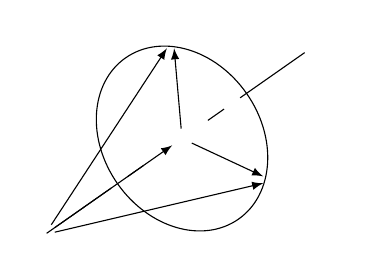
\begin{tikzpicture}
    [
        scale=2.5,
        % >=stealth,
        % point/.style = {draw, circle,  fill = black, inner sep = 1pt},
        % dot/.style   = {draw, circle,  fill = black, inner sep = .2pt},
    ]
    \def\rad{0.5}

    \node (origin) at (0,0)[]{};
    % \draw (origin) circle (\rad);
    \draw[rotate=125](origin) ellipse [x radius=0.5cm, y radius=0.4cm];
    % \draw[->] (p1) -- node (origin) {};

    \node (p) at +(-145:\rad*1.7){};
    \node (p1) at +(-145:\rad*1.8){};
    \node (p2) at +(35:\rad*1.8){};
    \node (p3) at +(95:\rad*1.02){};
    \node (p4) at +(-25:\rad*1.02){};

    % \node[double slit,slit height=0.15] (line) at (origin) {};

    \draw[-latex] (p) -- node (c)  {} (origin);
    \draw[-latex] (origin) -- (p3);
    \draw[-latex] (origin) -- (p4);
    \draw[-latex] (p) -- (p3);
    \draw[-latex] (p) -- (p4);
    \draw[dash pattern= on 1cm off 0.25cm on 0.25cm](p1)--(p2);
\end{tikzpicture}
    

\end{document}